\documentclass[11pt]{article}
% Supplementary Information of npj_manuscript.tex. Numbers marked \pd{...} come from
% pd_numbers.tex, fr_numbers.tex and ms_numbers.tex; tables from the same scripts.
\usepackage[letterpaper,margin=1in]{geometry}
\usepackage[T1]{fontenc}
\usepackage[utf8]{inputenc}
\usepackage{mathptmx}
\usepackage{amsmath,amssymb,bm}
\usepackage{microtype}
\usepackage{booktabs}
\usepackage{graphicx}
\usepackage{xcolor}
\usepackage{tabularx}
\usepackage[labelfont=bf,labelsep=period,font=small]{caption}
\usepackage[colorlinks=true,linkcolor=black,urlcolor=blue!50!black]{hyperref}
\hypersetup{pdftitle={Supplementary Information: Finding point defects in a model glass from atomic positions with neural networks},pdfauthor={Stacy Cheruto, Nicholaus Ladislaus, Abubakar Chilala, Gentille Uwera, Michel Sangwa, Boniface Godwin}}
\renewcommand{\figurename}{Supplementary Fig.}
\renewcommand{\tablename}{Supplementary Table}
\setlength{\textfloatsep}{12pt plus 2pt minus 2pt}
\makeatletter
\newcommand{\pd}[1]{\@ifundefined{pd@#1}{\textcolor{red}{[#1]}}{\csname pd@#1\endcsname}}
\newcommand{\pdset}[2]{\expandafter\gdef\csname pd@#1\endcsname{#2}}
\makeatother
\IfFileExists{pd_numbers.tex}{% written by make_report_numbers.py
\pdset{abl-diff-layers1}{6.2}
\pdset{abl-diff-layers2}{1.3}
\pdset{abl-diff-no-weights}{1.2}
\pdset{abl-diff-real-only}{0.0}
\pdset{abl-diff-scratch}{22.0}
\pdset{abl-label-layers1-interstitial}{0}
\pdset{abl-label-layers1-vacancy}{0}
\pdset{abl-label-layers2-interstitial}{0}
\pdset{abl-label-layers2-vacancy}{0}
\pdset{abl-label-no-weights-interstitial}{0}
\pdset{abl-label-no-weights-vacancy}{7}
\pdset{abl-label-real-only-interstitial}{17}
\pdset{abl-label-real-only-vacancy}{32}
\pdset{abl-label-reference-interstitial}{18}
\pdset{abl-label-reference-vacancy}{27}
\pdset{abl-label-scratch-interstitial}{0}
\pdset{abl-label-scratch-vacancy}{0}
\pdset{abl-layers1-all}{15.6}
\pdset{abl-layers1-antisite}{14.2}
\pdset{abl-layers1-frenkel}{13.8}
\pdset{abl-layers1-high}{17.3}
\pdset{abl-layers1-interstitial}{21.8}
\pdset{abl-layers1-low}{14.8}
\pdset{abl-layers1-sd}{1.5}
\pdset{abl-layers1-vacancy}{12.3}
\pdset{abl-layers2-all}{20.6}
\pdset{abl-layers2-antisite}{20.8}
\pdset{abl-layers2-frenkel}{21.3}
\pdset{abl-layers2-high}{23.1}
\pdset{abl-layers2-interstitial}{26.5}
\pdset{abl-layers2-low}{18.3}
\pdset{abl-layers2-sd}{2.4}
\pdset{abl-layers2-vacancy}{13.8}
\pdset{abl-lower-layers1}{3}
\pdset{abl-lower-layers2}{3}
\pdset{abl-lower-no-weights}{3}
\pdset{abl-lower-real-only}{2}
\pdset{abl-lower-scratch}{3}
\pdset{abl-no-weights-all}{42.7}
\pdset{abl-no-weights-antisite}{39.5}
\pdset{abl-no-weights-frenkel}{35.1}
\pdset{abl-no-weights-high}{43.5}
\pdset{abl-no-weights-interstitial}{31.0}
\pdset{abl-no-weights-low}{41.6}
\pdset{abl-no-weights-sd}{1.0}
\pdset{abl-no-weights-vacancy}{63.2}
\pdset{abl-real-only-ahead}{2.5}
\pdset{abl-real-only-all}{43.8}
\pdset{abl-real-only-antisite}{40.2}
\pdset{abl-real-only-behind}{2.5}
\pdset{abl-real-only-frenkel}{38.0}
\pdset{abl-real-only-high}{46.1}
\pdset{abl-real-only-interstitial}{30.8}
\pdset{abl-real-only-low}{42.1}
\pdset{abl-real-only-sd}{2.1}
\pdset{abl-real-only-vacancy}{64.7}
\pdset{abl-reference-all}{43.8}
\pdset{abl-reference-antisite}{41.7}
\pdset{abl-reference-frenkel}{38.7}
\pdset{abl-reference-high}{44.7}
\pdset{abl-reference-interstitial}{30.7}
\pdset{abl-reference-low}{43.2}
\pdset{abl-reference-sd}{0.8}
\pdset{abl-reference-vacancy}{63.0}
\pdset{abl-scratch-all}{21.9}
\pdset{abl-scratch-antisite}{24.2}
\pdset{abl-scratch-frenkel}{22.2}
\pdset{abl-scratch-high}{23.7}
\pdset{abl-scratch-interstitial}{26.8}
\pdset{abl-scratch-low}{18.7}
\pdset{abl-scratch-sd}{2.8}
\pdset{abl-scratch-vacancy}{14.3}
\pdset{abl-seeds}{three}
\pdset{abl-updates}{2,000}
\pdset{chance-antisite}{4}
\pdset{chance-frenkel}{5.4}
\pdset{chance-interstitial}{3}
\pdset{chance-max}{5}
\pdset{chance-min}{3}
\pdset{chance-vacancy}{2.9}
\pdset{exp-20k}{50.3}
\pdset{exp-60k}{54}
\pdset{exp-p-cal}{$p<0.001$}
\pdset{exp-p-length}{$p=0.001$}
\pdset{exp-uncal}{50.7}
\pdset{fin-by-all}{36--37}
\pdset{fin-by-none}{36--38}
\pdset{fin-by-one}{62--64}
\pdset{fin-cnn-all}{54.0}
\pdset{fin-cnn-antisite}{52.8}
\pdset{fin-cnn-frenkel}{38.4}
\pdset{fin-cnn-high}{54.4}
\pdset{fin-cnn-hours}{0.6}
\pdset{fin-cnn-interstitial}{51.2}
\pdset{fin-cnn-low}{53.5}
\pdset{fin-cnn-noshift}{12}
\pdset{fin-cnn-shift}{88}
\pdset{fin-cnn-size}{0.50}
\pdset{fin-cnn-vacancy}{69.7}
\pdset{fin-cnn3-all}{54.7}
\pdset{fin-cnn3-antisite}{54.0}
\pdset{fin-cnn3-frenkel}{38.7}
\pdset{fin-cnn3-hi}{59}
\pdset{fin-cnn3-interstitial}{51.5}
\pdset{fin-cnn3-lo}{51}
\pdset{fin-cnn3-p}{$p=0.86$}
\pdset{fin-cnn3-vacancy}{70.5}
\pdset{fin-egnn-all}{43.5}
\pdset{fin-egnn-antisite}{44.0}
\pdset{fin-egnn-frenkel}{35.1}
\pdset{fin-egnn-high}{43.9}
\pdset{fin-egnn-hours}{0.8}
\pdset{fin-egnn-interstitial}{29.7}
\pdset{fin-egnn-low}{42.9}
\pdset{fin-egnn-noshift}{0}
\pdset{fin-egnn-shift}{100}
\pdset{fin-egnn-size}{0.52}
\pdset{fin-egnn-vacancy}{63.2}
\pdset{fin-egnn3-all}{44.0}
\pdset{fin-egnn3-antisite}{45.5}
\pdset{fin-egnn3-frenkel}{32.7}
\pdset{fin-egnn3-hi}{48}
\pdset{fin-egnn3-interstitial}{30.0}
\pdset{fin-egnn3-lo}{40}
\pdset{fin-egnn3-p}{$p=1.00$}
\pdset{fin-egnn3-vacancy}{65.0}
\pdset{fin-lost-cnn}{38--42}
\pdset{fin-lost-pre}{43}
\pdset{fin-lost-tr}{34--41}
\pdset{fin-main-all}{54.0}
\pdset{fin-main-antisite}{49.0}
\pdset{fin-main-frenkel}{45.3}
\pdset{fin-main-interstitial}{50.0}
\pdset{fin-main-noshift}{0}
\pdset{fin-main-shift}{100}
\pdset{fin-main-size}{0.52}
\pdset{fin-main-vacancy}{69.5}
\pdset{fin-only-cnn}{114--122}
\pdset{fin-only-pre}{91}
\pdset{fin-only-tr}{110--116}
\pdset{fin-p-cnn}{$p<0.001$}
\pdset{fin-p-pre}{$p<0.001$}
\pdset{fin-p-tr}{$p<0.001$}
\pdset{fin-p-tr-cnn}{$p=0.49$--$0.91$}
\pdset{fin-p-tr-cnn-antisite}{0.33}
\pdset{fin-p-tr-cnn-frenkel}{0.25}
\pdset{fin-p-tr-cnn-interstitial}{0.04}
\pdset{fin-p-tr-cnn-vacancy}{0.12}
\pdset{fin-pair-all}{55.2}
\pdset{fin-pair-antisite}{55.5}
\pdset{fin-pair-frenkel}{41.3}
\pdset{fin-pair-hi}{59}
\pdset{fin-pair-interstitial}{51.5}
\pdset{fin-pair-lo}{51}
\pdset{fin-pair-p}{$p=0.090$}
\pdset{fin-pair-vacancy}{69.0}
\pdset{fin-pre-all}{50.3}
\pdset{fin-pre-antisite}{46.5}
\pdset{fin-pre-frenkel}{36.7}
\pdset{fin-pre-interstitial}{47.5}
\pdset{fin-pre-noshift}{0}
\pdset{fin-pre-shift}{100}
\pdset{fin-pre-size}{0.52}
\pdset{fin-pre-vacancy}{67.0}
\pdset{fin-report-all}{55.2}
\pdset{fin-report-antisite}{55.0}
\pdset{fin-report-frenkel}{41.3}
\pdset{fin-report-hi}{59}
\pdset{fin-report-interstitial}{51.0}
\pdset{fin-report-lo}{51}
\pdset{fin-report-p}{$p=0.30$}
\pdset{fin-report-vacancy}{70.0}
\pdset{fin-six-all}{55.1}
\pdset{fin-six-antisite}{56.0}
\pdset{fin-six-frenkel}{41.3}
\pdset{fin-six-hi}{59}
\pdset{fin-six-interstitial}{49.5}
\pdset{fin-six-lo}{51}
\pdset{fin-six-p}{$p=0.58$}
\pdset{fin-six-vacancy}{70.0}
\pdset{fin-three-all}{54.1}
\pdset{fin-three-antisite}{54.5}
\pdset{fin-three-frenkel}{40.7}
\pdset{fin-three-hi}{58}
\pdset{fin-three-interstitial}{50.0}
\pdset{fin-three-lo}{50}
\pdset{fin-three-p}{$p=0.77$}
\pdset{fin-three-vacancy}{68.0}
\pdset{fin-tr-all}{53.6}
\pdset{fin-tr-antisite}{54.2}
\pdset{fin-tr-frenkel}{42.0}
\pdset{fin-tr-high}{53.9}
\pdset{fin-tr-hours}{0.6}
\pdset{fin-tr-interstitial}{48.3}
\pdset{fin-tr-low}{53.3}
\pdset{fin-tr-noshift}{0}
\pdset{fin-tr-shift}{100}
\pdset{fin-tr-size}{0.58}
\pdset{fin-tr-vacancy}{67.2}
\pdset{fin-tr3-all}{54.5}
\pdset{fin-tr3-antisite}{56.5}
\pdset{fin-tr3-frenkel}{42.7}
\pdset{fin-tr3-hi}{58}
\pdset{fin-tr3-interstitial}{48.0}
\pdset{fin-tr3-lo}{51}
\pdset{fin-tr3-p}{$p=0.44$}
\pdset{fin-tr3-vacancy}{68.0}
\pdset{fother-found-bonds}{26.2}
\pdset{fother-found-bonds-hi}{36}
\pdset{fother-found-bonds-lo}{17}
\pdset{fother-found-energy}{31}
\pdset{fother-found-energy-hi}{41}
\pdset{fother-found-energy-lo}{22}
\pdset{fother-found-finder}{44}
\pdset{fother-found-finder-hi}{55}
\pdset{fother-found-finder-lo}{33}
\pdset{fother-found-geometry}{20.2}
\pdset{fother-found-geometry-hi}{28}
\pdset{fother-found-geometry-lo}{12}
\pdset{fother-n}{84}
\pdset{fother-p-found-energy}{$p=0.071$}
\pdset{fother-p-restored-energy}{$p=0.77$}
\pdset{fother-restored-bonds}{1.2}
\pdset{fother-restored-bonds-hi}{4}
\pdset{fother-restored-bonds-lo}{0}
\pdset{fother-restored-ceiling}{27.4}
\pdset{fother-restored-ceiling-hi}{38}
\pdset{fother-restored-ceiling-lo}{18}
\pdset{fother-restored-energy}{6}
\pdset{fother-restored-energy-hi}{11}
\pdset{fother-restored-energy-lo}{1}
\pdset{fother-restored-finder}{8.3}
\pdset{fother-restored-finder-hi}{14}
\pdset{fother-restored-finder-lo}{3}
\pdset{fother-restored-geometry}{0}
\pdset{fother-restored-geometry-hi}{4}
\pdset{fother-restored-geometry-lo}{0}
\pdset{found-best-antisite}{31.5}
\pdset{found-best-frenkel}{32.7}
\pdset{found-best-interstitial}{28}
\pdset{found-best-vacancy}{47.5}
\pdset{found-bonds-antisite}{31.5}
\pdset{found-bonds-frenkel}{27.3}
\pdset{found-bonds-interstitial}{28}
\pdset{found-bonds-max}{31.5}
\pdset{found-bonds-min}{27.3}
\pdset{found-bonds-vacancy}{29}
\pdset{found-energy-antisite}{29}
\pdset{found-energy-frenkel}{32.7}
\pdset{found-energy-interstitial}{28}
\pdset{found-energy-max}{32.7}
\pdset{found-energy-min}{28}
\pdset{found-energy-vacancy}{29.5}
\pdset{found-finder-antisite}{49}
\pdset{found-finder-frenkel}{45.3}
\pdset{found-finder-interstitial}{50}
\pdset{found-finder-vacancy}{69.5}
\pdset{found-geometry-antisite}{16.5}
\pdset{found-geometry-frenkel}{26.7}
\pdset{found-geometry-interstitial}{15}
\pdset{found-geometry-max}{47.5}
\pdset{found-geometry-min}{15}
\pdset{found-geometry-vacancy}{47.5}
\pdset{fp-n-anti}{35}
\pdset{fp-n-close}{27}
\pdset{fp-n-complex}{19}
\pdset{fp-n-none}{3}
\pdset{fp-n-pair}{66}
\pdset{fp-n-pair-pure}{40}
\pdset{fpair-found-bonds}{28.8}
\pdset{fpair-found-bonds-hi}{40}
\pdset{fpair-found-bonds-lo}{19}
\pdset{fpair-found-energy}{34.8}
\pdset{fpair-found-energy-hi}{47}
\pdset{fpair-found-energy-lo}{24}
\pdset{fpair-found-finder}{47}
\pdset{fpair-found-finder-hi}{59}
\pdset{fpair-found-finder-lo}{35}
\pdset{fpair-found-geometry}{34.8}
\pdset{fpair-found-geometry-hi}{47}
\pdset{fpair-found-geometry-lo}{24}
\pdset{fpair-n}{66}
\pdset{fpair-p-found-energy}{$p=0.15$}
\pdset{fpair-p-restored-energy}{$p=0.18$}
\pdset{fpair-restored-bonds}{1.5}
\pdset{fpair-restored-bonds-hi}{5}
\pdset{fpair-restored-bonds-lo}{0}
\pdset{fpair-restored-ceiling}{60.6}
\pdset{fpair-restored-ceiling-hi}{71}
\pdset{fpair-restored-ceiling-lo}{49}
\pdset{fpair-restored-energy}{9.1}
\pdset{fpair-restored-energy-hi}{17}
\pdset{fpair-restored-energy-lo}{3}
\pdset{fpair-restored-finder}{18.2}
\pdset{fpair-restored-finder-hi}{28}
\pdset{fpair-restored-finder-lo}{10}
\pdset{fpair-restored-geometry}{0}
\pdset{fpair-restored-geometry-hi}{5}
\pdset{fpair-restored-geometry-lo}{0}
\pdset{frenkel-exact-energy}{7}
\pdset{frenkel-exact-finder}{21}
\pdset{gap-finder-energy-max}{40}
\pdset{gap-finder-energy-min}{20}
\pdset{glass-auc}{0.75}
\pdset{glass-clean-cal}{2}
\pdset{glass-clean-raw}{68}
\pdset{glass-def-cal}{28.7}
\pdset{lead-found-antisite}{18}
\pdset{lead-found-frenkel}{13}
\pdset{lead-found-interstitial}{22}
\pdset{lead-found-max}{22}
\pdset{lead-found-min}{18}
\pdset{lead-found-vacancy}{22}
\pdset{lead-restored-antisite}{22}
\pdset{lead-restored-frenkel}{5}
\pdset{lead-restored-interstitial}{16}
\pdset{lead-restored-vacancy}{13}
\pdset{n-antisite}{200}
\pdset{n-frenkel}{150}
\pdset{n-interstitial}{200}
\pdset{n-test}{750}
\pdset{n-tests-family}{12}
\pdset{n-vacancy}{200}
\pdset{occ-anti}{71}
\pdset{occ-anti-pairlike}{22}
\pdset{occ-int}{95.5}
\pdset{occ-undone}{50}
\pdset{occ-undone-n}{50}
\pdset{occ-vac}{93}
\pdset{p-found-bonds-antisite}{<0.001}
\pdset{p-found-bonds-frenkel}{<0.001}
\pdset{p-found-bonds-interstitial}{<0.001}
\pdset{p-found-bonds-vacancy}{<0.001}
\pdset{p-found-energy-antisite}{<0.001}
\pdset{p-found-energy-frenkel}{0.014}
\pdset{p-found-energy-interstitial}{<0.001}
\pdset{p-found-energy-vacancy}{<0.001}
\pdset{p-found-geometry-antisite}{<0.001}
\pdset{p-found-geometry-frenkel}{0.002}
\pdset{p-found-geometry-interstitial}{<0.001}
\pdset{p-found-geometry-vacancy}{<0.001}
\pdset{p-restored-bonds-antisite}{<0.001}
\pdset{p-restored-bonds-frenkel}{<0.001}
\pdset{p-restored-bonds-interstitial}{<0.001}
\pdset{p-restored-bonds-vacancy}{<0.001}
\pdset{p-restored-energy-antisite}{<0.001}
\pdset{p-restored-energy-frenkel}{0.169}
\pdset{p-restored-energy-interstitial}{<0.001}
\pdset{p-restored-energy-vacancy}{<0.001}
\pdset{p-restored-geometry-antisite}{<0.001}
\pdset{p-restored-geometry-frenkel}{<0.001}
\pdset{p-restored-geometry-interstitial}{<0.001}
\pdset{p-restored-geometry-vacancy}{<0.001}
\pdset{p-worst-found}{p<0.001}
\pdset{p-worst-restored}{p<0.001}
\pdset{praw-found-bonds-antisite}{<0.001}
\pdset{praw-found-bonds-frenkel}{<0.001}
\pdset{praw-found-bonds-interstitial}{<0.001}
\pdset{praw-found-bonds-vacancy}{<0.001}
\pdset{praw-found-energy-antisite}{<0.001}
\pdset{praw-found-energy-frenkel}{0.014}
\pdset{praw-found-energy-interstitial}{<0.001}
\pdset{praw-found-energy-vacancy}{<0.001}
\pdset{praw-found-geometry-antisite}{<0.001}
\pdset{praw-found-geometry-frenkel}{<0.001}
\pdset{praw-found-geometry-interstitial}{<0.001}
\pdset{praw-found-geometry-vacancy}{<0.001}
\pdset{praw-restored-bonds-antisite}{<0.001}
\pdset{praw-restored-bonds-frenkel}{<0.001}
\pdset{praw-restored-bonds-interstitial}{<0.001}
\pdset{praw-restored-bonds-vacancy}{<0.001}
\pdset{praw-restored-energy-antisite}{<0.001}
\pdset{praw-restored-energy-frenkel}{0.169}
\pdset{praw-restored-energy-interstitial}{<0.001}
\pdset{praw-restored-energy-vacancy}{<0.001}
\pdset{praw-restored-geometry-antisite}{<0.001}
\pdset{praw-restored-geometry-frenkel}{<0.001}
\pdset{praw-restored-geometry-interstitial}{<0.001}
\pdset{praw-restored-geometry-vacancy}{<0.001}
\pdset{press-antisite}{16}
\pdset{press-antisite-hi}{22}
\pdset{press-antisite-lo}{11}
\pdset{press-antisite-rule}{lowest}
\pdset{press-frenkel}{10.7}
\pdset{press-frenkel-hi}{16}
\pdset{press-frenkel-lo}{6}
\pdset{press-frenkel-rule}{lowest}
\pdset{press-interstitial}{19}
\pdset{press-interstitial-hi}{25}
\pdset{press-interstitial-lo}{14}
\pdset{press-interstitial-rule}{most unusual}
\pdset{press-max}{19}
\pdset{press-min}{8.5}
\pdset{press-p-antisite}{$p<0.001$}
\pdset{press-p-frenkel}{$p<0.001$}
\pdset{press-p-interstitial}{$p<0.001$}
\pdset{press-p-vacancy}{$p<0.001$}
\pdset{press-ref-a}{6.5\pm5.4}
\pdset{press-ref-b}{2.9\pm5.4}
\pdset{press-vacancy}{8.5}
\pdset{press-vacancy-hi}{12}
\pdset{press-vacancy-lo}{5}
\pdset{press-vacancy-rule}{lowest}
\pdset{press-val-highest}{21}
\pdset{press-val-unusual}{21.5}
\pdset{presscell-antisite}{15}
\pdset{presscell-antisite-hi}{20}
\pdset{presscell-antisite-lo}{10}
\pdset{presscell-antisite-rule}{lowest}
\pdset{presscell-frenkel}{7.3}
\pdset{presscell-frenkel-hi}{12}
\pdset{presscell-frenkel-lo}{3}
\pdset{presscell-frenkel-rule}{lowest}
\pdset{presscell-interstitial}{16.5}
\pdset{presscell-interstitial-hi}{23}
\pdset{presscell-interstitial-lo}{10}
\pdset{presscell-interstitial-rule}{highest}
\pdset{presscell-max}{16.5}
\pdset{presscell-min}{7}
\pdset{presscell-p-antisite}{$p<0.001$}
\pdset{presscell-p-frenkel}{$p<0.001$}
\pdset{presscell-p-interstitial}{$p<0.001$}
\pdset{presscell-p-vacancy}{$p<0.001$}
\pdset{presscell-vacancy}{7}
\pdset{presscell-vacancy-hi}{10}
\pdset{presscell-vacancy-lo}{4}
\pdset{presscell-vacancy-rule}{lowest}
\pdset{ratio-finder-energy-max}{2.4}
\pdset{ratio-finder-energy-min}{1.7}
\pdset{repair-overlap-1}{1--40}
\pdset{repair-overlap-10}{50--73}
\pdset{repair-removed-v1}{7--9}
\pdset{repair-removed-v2}{13--16}
\pdset{restored-best-antisite}{8}
\pdset{restored-best-frenkel}{7.3}
\pdset{restored-best-interstitial}{21.5}
\pdset{restored-best-vacancy}{40.5}
\pdset{restored-bonds-antisite}{7.5}
\pdset{restored-bonds-frenkel}{1.3}
\pdset{restored-bonds-interstitial}{21.5}
\pdset{restored-bonds-max}{22}
\pdset{restored-bonds-min}{1.3}
\pdset{restored-bonds-vacancy}{22}
\pdset{restored-ceiling-antisite}{68.5}
\pdset{restored-ceiling-frenkel}{42}
\pdset{restored-ceiling-interstitial}{80}
\pdset{restored-ceiling-max}{80}
\pdset{restored-ceiling-min}{42}
\pdset{restored-ceiling-vacancy}{67}
\pdset{restored-energy-antisite}{8}
\pdset{restored-energy-frenkel}{7.3}
\pdset{restored-energy-interstitial}{21}
\pdset{restored-energy-max}{26}
\pdset{restored-energy-min}{7.3}
\pdset{restored-energy-vacancy}{26}
\pdset{restored-finder-antisite}{30}
\pdset{restored-finder-frenkel}{12.7}
\pdset{restored-finder-interstitial}{38}
\pdset{restored-finder-vacancy}{53.5}
\pdset{restored-geometry-antisite}{1.5}
\pdset{restored-geometry-frenkel}{0}
\pdset{restored-geometry-interstitial}{8.5}
\pdset{restored-geometry-max}{40.5}
\pdset{restored-geometry-min}{0}
\pdset{restored-geometry-vacancy}{40.5}
\pdset{seed-agree}{88}
\pdset{seed-by-all}{37.7}
\pdset{seed-by-none}{50.1}
\pdset{seed-ensemble}{45.1}
\pdset{seed-ref-runs}{43.2, 43.6 and 44.7}
\pdset{stab-cnn-clipped}{85}
\pdset{stab-cnn-gspikes}{0}
\pdset{stab-cnn-largest}{6.3--8.1}
\pdset{stab-cnn-lspikes}{0}
\pdset{stab-cnn-median}{1.6--1.8}
\pdset{stab-cnn-runs}{3}
\pdset{stab-cnn-updates}{20,000}
\pdset{stab-egnn-clipped}{85--88}
\pdset{stab-egnn-cut}{85--96}
\pdset{stab-egnn-first}{7,818 and 9,704}
\pdset{stab-egnn-gspikes}{71--131}
\pdset{stab-egnn-largest}{55--82}
\pdset{stab-egnn-lspikes}{14--34}
\pdset{stab-egnn-median}{1.5--1.6}
\pdset{stab-egnn-runs}{3}
\pdset{stab-egnn-updates}{20,000}
\pdset{stab-max-ratio}{46}
\pdset{stab-not-finite}{0}
\pdset{stab-now-clipped}{1--3}
\pdset{stab-now-first}{647 and 731}
\pdset{stab-now-gspikes}{3--4}
\pdset{stab-now-largest}{6.2--6.7}
\pdset{stab-now-lspikes}{5--11}
\pdset{stab-now-median}{0.31--0.34}
\pdset{stab-now-runs}{2}
\pdset{stab-now-updates}{2,000}
\pdset{stab-ref-clipped}{95--96}
\pdset{stab-ref-first}{395 and 811}
\pdset{stab-ref-gspikes}{9--32}
\pdset{stab-ref-largest}{38--86}
\pdset{stab-ref-lspikes}{1--13}
\pdset{stab-ref-median}{2.0--2.5}
\pdset{stab-ref-runs}{3}
\pdset{stab-ref-updates}{2,000}
\pdset{stab-runs}{23}
\pdset{stab-scr-clipped}{92--93}
\pdset{stab-scr-gspikes}{0}
\pdset{stab-scr-largest}{4.1--5.2}
\pdset{stab-scr-lspikes}{0}
\pdset{stab-scr-median}{1.4--1.5}
\pdset{stab-scr-runs}{3}
\pdset{stab-scr-updates}{2,000}
\pdset{stab-tr-clipped}{40--50}
\pdset{stab-tr-gspikes}{0}
\pdset{stab-tr-largest}{4.9--5.5}
\pdset{stab-tr-lspikes}{0--1}
\pdset{stab-tr-median}{0.9--1.0}
\pdset{stab-tr-runs}{3}
\pdset{stab-tr-updates}{20,000}
\pdset{vacA-found-bonds}{40.9}
\pdset{vacA-found-bonds-hi}{49}
\pdset{vacA-found-bonds-lo}{33}
\pdset{vacA-found-energy}{40.2}
\pdset{vacA-found-energy-hi}{49}
\pdset{vacA-found-energy-lo}{31}
\pdset{vacA-found-finder}{69.3}
\pdset{vacA-found-finder-hi}{77}
\pdset{vacA-found-finder-lo}{61}
\pdset{vacA-found-geometry}{56.7}
\pdset{vacA-found-geometry-hi}{66}
\pdset{vacA-found-geometry-lo}{47}
\pdset{vacA-n}{127}
\pdset{vacA-p-found-energy}{$p<0.001$}
\pdset{vacA-p-restored-energy}{$p<0.001$}
\pdset{vacA-restored-bonds}{29.1}
\pdset{vacA-restored-bonds-hi}{38}
\pdset{vacA-restored-bonds-lo}{21}
\pdset{vacA-restored-ceiling}{58.3}
\pdset{vacA-restored-ceiling-hi}{67}
\pdset{vacA-restored-ceiling-lo}{49}
\pdset{vacA-restored-energy}{34.6}
\pdset{vacA-restored-energy-hi}{43}
\pdset{vacA-restored-energy-lo}{26}
\pdset{vacA-restored-finder}{49.6}
\pdset{vacA-restored-finder-hi}{59}
\pdset{vacA-restored-finder-lo}{40}
\pdset{vacA-restored-geometry}{47.2}
\pdset{vacA-restored-geometry-hi}{57}
\pdset{vacA-restored-geometry-lo}{38}
\pdset{vacB-found-bonds}{8.2}
\pdset{vacB-found-bonds-hi}{15}
\pdset{vacB-found-bonds-lo}{3}
\pdset{vacB-found-energy}{11}
\pdset{vacB-found-energy-hi}{18}
\pdset{vacB-found-energy-lo}{4}
\pdset{vacB-found-finder}{69.9}
\pdset{vacB-found-finder-hi}{80}
\pdset{vacB-found-finder-lo}{59}
\pdset{vacB-found-geometry}{31.5}
\pdset{vacB-found-geometry-hi}{43}
\pdset{vacB-found-geometry-lo}{20}
\pdset{vacB-n}{73}
\pdset{vacB-p-found-energy}{$p<0.001$}
\pdset{vacB-p-restored-energy}{$p<0.001$}
\pdset{vacB-restored-bonds}{9.6}
\pdset{vacB-restored-bonds-hi}{17}
\pdset{vacB-restored-bonds-lo}{4}
\pdset{vacB-restored-ceiling}{82.2}
\pdset{vacB-restored-ceiling-hi}{90}
\pdset{vacB-restored-ceiling-lo}{73}
\pdset{vacB-restored-energy}{11}
\pdset{vacB-restored-energy-hi}{18}
\pdset{vacB-restored-energy-lo}{4}
\pdset{vacB-restored-finder}{60.3}
\pdset{vacB-restored-finder-hi}{71}
\pdset{vacB-restored-finder-lo}{49}
\pdset{vacB-restored-geometry}{28.8}
\pdset{vacB-restored-geometry-hi}{40}
\pdset{vacB-restored-geometry-lo}{18}
\pdset{vacancy-closed}{40}
\pdset{vacancy-open}{60}
}{}
\IfFileExists{fr_numbers.tex}{% written by make_final_numbers.py
\pdset{feat-atoms}{4,159}
\pdset{knn-den}{31}
\pdset{knn-fin}{43}
\pdset{noise-bonds-0}{28.9}
\pdset{noise-bonds-100}{8}
\pdset{noise-bonds-20}{29.2}
\pdset{noise-bonds-50}{26.3}
\pdset{noise-cell-0}{26.4}
\pdset{noise-cell-100}{8.9}
\pdset{noise-cell-20}{22.8}
\pdset{noise-cell-50}{15.7}
\pdset{noise-cnn-0}{53.5}
\pdset{noise-cnn-100}{10.1}
\pdset{noise-cnn-20}{35.1}
\pdset{noise-cnn-50}{17.6}
\pdset{noise-drop-fin}{16}
\pdset{noise-energy-0}{29.6}
\pdset{noise-energy-100}{3.6}
\pdset{noise-energy-20}{10.4}
\pdset{noise-energy-50}{3.5}
\pdset{noise-fin-0}{54}
\pdset{noise-fin-100}{11.3}
\pdset{noise-fin-20}{38.1}
\pdset{noise-fin-50}{18.8}
\pdset{noise-max-last}{12.7}
\pdset{noise-scr-0}{43.9}
\pdset{noise-scr-100}{12.7}
\pdset{noise-scr-20}{42.4}
\pdset{noise-scr-50}{34.8}
\pdset{noise-tr-0}{53.7}
\pdset{noise-tr-100}{3.5}
\pdset{noise-tr-20}{31.1}
\pdset{noise-tr-50}{7.1}
\pdset{size-cnn}{498,309}
\pdset{size-den}{530,696}
\pdset{size-egnn}{523,021}
\pdset{size-layer}{117,890}
\pdset{size-tr}{576,677}
\pdset{split-test-all}{54}
\pdset{split-test-antisite}{49}
\pdset{split-test-ce}{0.109}
\pdset{split-test-frenkel}{45.3}
\pdset{split-test-interstitial}{50}
\pdset{split-test-vacancy}{69.5}
\pdset{split-test-wce}{0.371}
\pdset{split-train-all}{50.5}
\pdset{split-train-antisite}{50.5}
\pdset{split-train-ce}{0.111}
\pdset{split-train-frenkel}{43}
\pdset{split-train-interstitial}{44}
\pdset{split-train-vacancy}{64.5}
\pdset{split-train-wce}{0.396}
\pdset{split-val-all}{52.2}
\pdset{split-val-antisite}{54.5}
\pdset{split-val-ce}{0.109}
\pdset{split-val-frenkel}{47.8}
\pdset{split-val-interstitial}{48.5}
\pdset{split-val-vacancy}{56.5}
\pdset{split-val-wce}{0.381}
}{}
\IfFileExists{ms_numbers.tex}{% written by make_manuscript_tables.py
\pdset{ph-as-above}{89}
\pdset{ph-as-below}{11}
\pdset{ph-as-e}{2.8}
\pdset{ph-fp-above}{91}
\pdset{ph-fp-e}{3.2}
\pdset{ph-int-e}{-3.0}
\pdset{ph-int-e-free}{-3.4}
\pdset{ph-int-nn}{0.85}
\pdset{ph-int-nn-free}{0.87}
\pdset{ph-moved-max}{44}
\pdset{ph-moved-min}{14}
\pdset{ph-open-free}{0.63}
\pdset{ph-open-free-p95}{0.70}
\pdset{ph-vac-open-after}{0.74}
\pdset{ph-vac-open-before}{0.87}
}{}
\newcommand{\ci}[1]{{\scriptsize[\pd{#1-lo}, \pd{#1-hi}]}}

\begin{document}
\begin{center}
{\Large\bfseries Supplementary Information\par}
\vspace{6pt}
{\large Finding point defects in a model glass from atomic positions with neural networks\par}
\vspace{6pt}
Stacy Cheruto, Nicholaus Ladislaus, Abubakar Chilala, Gentille Uwera, Michel Sangwa and Boniface Godwin
\end{center}

\noindent All numbers are computed from the result files in the repository (\url{https://github.com/chilalaabubakar/IDL-PROJECT}, branch \texttt{dabo-point-defects}). Shares are in \%, with 95\% bootstrap intervals over the test glasses in brackets where given.

\section*{Supplementary Figures}

\begin{figure}[h]
\centering
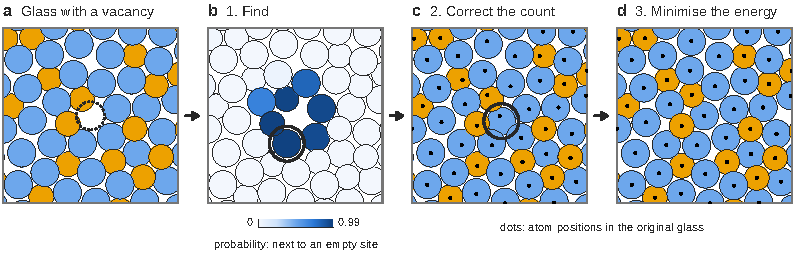
\includegraphics[width=0.95\linewidth]{figures/pd_fig2_pipeline.pdf}
\caption{\textbf{Finding and repairing one test vacancy.} \textbf{a} The relaxed glass; the dotted circle marks where the atom was removed, which the methods are not told. \textbf{b} The finder's probability that each atom is next to an empty site; the flagged atom is ringed. \textbf{c} An atom of the missing species is put at the most open point near the flagged atom. \textbf{d} After energy minimisation every atom sits on its position in the original glass (dots); in \textbf{c} the atoms around the defect are still off theirs.}
\label{fig:pipeline}
\end{figure}

\begin{figure}[h]
\centering
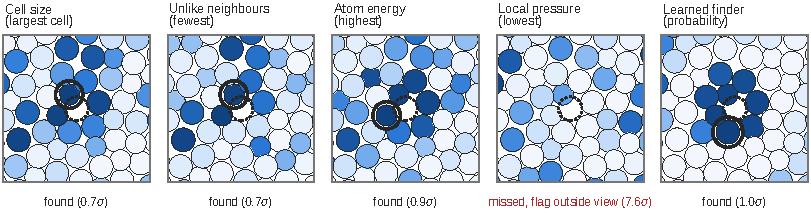
\includegraphics[width=\linewidth]{figures/fr_fig_baselines.pdf}
\caption{\textbf{Output of every method on the same test vacancy.} The dotted circle marks where the atom was removed (not shown to the methods). Atoms are coloured by how suspicious each method finds them (rank within the glass, dark = most); the ringed atom is the one flagged. In this typical example three of the four measures also find the defect; local pressure flags an atom $7.6\sigma$ away.}
\label{fig:baselines}
\end{figure}

\begin{figure}[h]
\centering
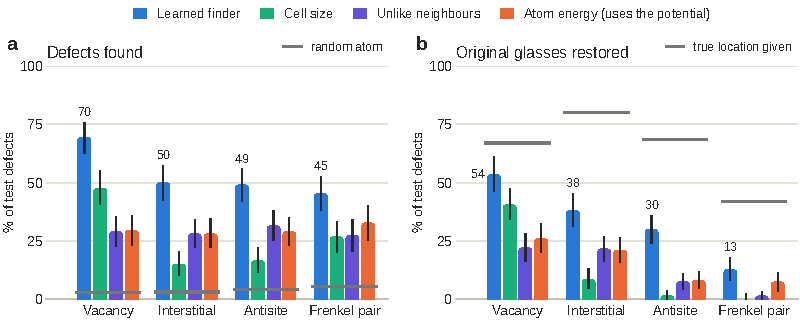
\includegraphics[width=0.9\linewidth]{figures/pd_fig3_results.pdf}
\caption{\textbf{Test results by method.} \textbf{a} Defects found: the flagged atom is within $1.5\sigma$ of the defect. Grey lines: a randomly chosen atom. \textbf{b} Original glasses restored after correcting the atoms at the flagged atom and minimising the energy. Grey lines: the same with the true location given. Whiskers: 95\% intervals. The first three methods use no potential to flag the atom. The values are those of Table~1 of the main text.}
\label{fig:results}
\end{figure}

\begin{figure}[h]
\centering
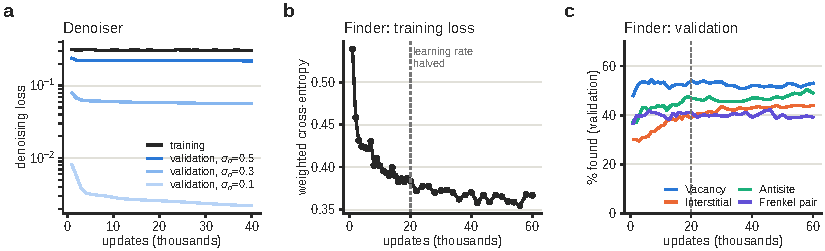
\includegraphics[width=\linewidth]{figures/fr_fig_training.pdf}
\caption{\textbf{Training and validation.} \textbf{a} Denoiser: training loss (averaged over all noise levels, so it stays near the noise floor) and validation loss at three fixed noise levels. \textbf{b} Finder: class-weighted training loss, mean over 1,000 updates. \textbf{c} Finder: share of validation defects found (first 200 per type, uncalibrated, including the Frenkel pairs that undid themselves).}
\label{fig:training}
\end{figure}

\clearpage
\section*{Supplementary Tables}

% written by make_manuscript_tables.py
\begin{table}[h]
\centering
\caption{\textbf{The relaxed defects on the test glasses.} Medians with the interquartile range in brackets. Energies are compared with the original glass, so only defects that keep the number of atoms are listed.}
\label{tab:physics}
\footnotesize
\begin{tabular}{@{}lcccc@{}}
\toprule
 & Vacancy & Interstitial & Frenkel pair & Antisite \\
\midrule
Real defects in the test & 200 & 200 & 150 & 200 \\
Other atoms moved $>0.1\sigma$ & 14 [3, 43] & 22 [12, 40] & 44 [21, 69] & 28 [15, 55] \\
Largest move of another atom ($\sigma$) & 0.33 [0.15, 0.65] & 0.32 [0.23, 0.42] & 0.64 [0.42, 0.90] & 0.42 [0.34, 0.55] \\
Energy above the original ($\epsilon$) & -- & -- & 3.2 [1.5, 5.0] & 2.8 [1.4, 4.3] \\
\bottomrule
\end{tabular}
\end{table}

% written by make_manuscript_tables.py
\begin{table}[h]
\centering
\caption{\textbf{Site-occupancy check.} Top: share of defects of known kind that the occupancy rule classifies as expected (\%; last column: Frenkel pairs that undid themselves classified as no defect). Bottom: classes of the 150 real test Frenkel pairs.}
\label{tab:occupancy}
\footnotesize
\begin{tabular}{@{}lcccc@{}}
\toprule
Split & Vacancy & Interstitial & Antisite & Undone Frenkel pairs \\
\midrule
Test & 93.0 & 95.5 & 71.0 & 50/50 \\
Validation & 91.5 & 94.0 & 67.5 & 65/65 \\
\bottomrule
\end{tabular}

\vspace{6pt}
\begin{tabular}{@{}lc@{}}
\toprule
Class of the relaxed Frenkel pair & Test defects \\
\midrule
Frenkel pair & 66 \\
Close pair & 27 \\
Antisite-like & 35 \\
Complex & 19 \\
No defect & 3 \\
\bottomrule
\end{tabular}
\end{table}

% copy of fr_table_models.tex written by make_manuscript_tables.py
% Model description table of final_report.tex, laid out as Table 1 of Henderson et al.,
% Nucleic Acids Research 2019: model, hidden layers, parameters and hyper-parameters tried.
\begin{table}[t]
\centering
\caption{\textbf{Models explored in this study.} For each: model name, hidden layers and, in column 3, the parameters and hyper-parameters varied within each group, with the values tried in brackets and the value of the final model in bold. $N\times\{\text{layer}\}$ is a layer repeated $N$ times. Fixed for all: 128 features, batches of 16 glasses, AdamW with learning rate $2\times10^{-4}$, gradient norm cut at 1, moving average of the weights 0.999. Output shapes and parameter counts are in Supplementary Table~\ref{tab:shapes}.}
\label{tab:models}
\footnotesize\setlength{\tabcolsep}{4pt}
\begin{tabularx}{\linewidth}{@{}l>{\raggedright\arraybackslash}X>{\raggedright\arraybackslash}p{2.05in}@{}}
\toprule
Model & Hidden layers & Parameters/hyper-parameters \\
\midrule
4layerEGNN\_Denoiser & $1\times\{$embedding$\}$, $4\times\{$EGNN layer$\}$, vector head & Noise level $\sigma_n\sim\mathcal U(0.001,1)$; updates (40,000) \\
\addlinespace
4layerEGNN\_Finder & $1\times\{$embedding$\}$, $\mathbf{4}\times\{$EGNN layer$\}$, $1\times\{$Dense 128, Dense 5$\}$ & Starting weights (\textbf{denoiser}, random) \\
2layerEGNN\_Finder & $1\times\{$embedding$\}$, $2\times\{$EGNN layer$\}$, $1\times\{$Dense 128, Dense 5$\}$ & Class weights $w_c$ (\textbf{frequency}$^{\mathbf{-1/2}}$, none) \\
1layerEGNN\_Finder & $1\times\{$embedding$\}$, $1\times\{$EGNN layer$\}$, $1\times\{$Dense 128, Dense 5$\}$ & Frenkel pairs in training (\textbf{all}, real only) \\
 & & Updates (2,000, 20,000, \textbf{60,000}); learning rate after 20,000 updates ($2\times10^{-4}$, $\mathbf{1\times10^{-4}}$); calibration (none, \textbf{logit adjustment}); seeds (\textbf{0}, 1, 2) \\
\addlinespace
4layerTransformer\_Finder & $1\times\{$embedding$\}$, $4\times\{$attention with distance bias (8 heads), feed-forward$\}$, $1\times\{$Dense 128, Dense 5$\}$ & Starting weights (random); learning-rate warm-up (1,000 updates); updates (20,000); seeds (0, 1, 2) \\
5levelUNet\_Finder & $1\times\{$draw glass as picture$\}$, $5\times\{$Conv, Conv, pooling$\}$, $4\times\{$upsample, Conv, Conv$\}$, $1\times\{$Dense 64, Dense 5$\}$ & Starting weights (random); training augmentation (8 turns and mirrors, random shift); test-time average over 8; updates (20,000); seeds (0, 1, 2) \\
\addlinespace
4layerEGNN\_Repair & as 4layerEGNN\_Denoiser & Weight of displaced atoms (1, \textbf{11}); noise level ($\mathcal U(0.001,0.5)$, \textbf{log-uniform (0.001, 0.3)}); updates ($2\times20{,}000$) \\
\bottomrule
\end{tabularx}
\end{table}

% written by make_final_numbers.py
\begin{table}[t]
\centering
\caption{Output shape and number of parameters of every block, for one batch of 16 glasses of 256 atoms (shapes: glasses $\times$ atoms $\times$ features; for the CNN: glasses $\times$ channels $\times$ pixels $\times$ pixels). The neighbour graph holds up to 64 neighbours per atom (about 22 are within the cutoff). Measured on the trained networks.}
\label{tab:shapes}
\scriptsize\setlength{\tabcolsep}{4pt}
\begin{tabularx}{\linewidth}{@{}>{\raggedright\arraybackslash}Xlr@{}}
\toprule
Block & Output shape & Parameters \\
\midrule
\multicolumn{3}{@{}l}{\emph{EGNN finder} (the denoiser is the same with a noise-level input and the vector head)} \\
Input: positions, species & $16\times256\times2$, $16\times256$ & 0 \\
Neighbour graph and distance features (16 radial functions) & $16\times256\times64\times16$ & 0 \\
Input embedding (denoiser: with noise level) & $16\times256\times128$ & 34,304 (59,136) \\
$4\times$\{EGNN layer\}: features $h$, vector $v$ & $16\times256\times128$, $16\times256\times2$ & $4\times117,890$ \\
Role head \{Dense 128, Dense 5\} (denoiser: vector head, sum of $v$) & $16\times256\times5$ ($16\times256\times2$) & 17,157 (0) \\
\emph{Total} & & 523,021 (530,696) \\
\addlinespace
\multicolumn{3}{@{}l}{\emph{Transformer finder}} \\
Embedding: species, and neighbours of each species by distance & $16\times256\times128$ & 20,992 \\
Pair features from every distance (32 radial functions) & $16\times256\times256\times64$ & 6,272 \\
$4\times$\{attention with distance bias (8 heads), feed-forward 256\} & $16\times256\times128$ & $4\times133,000$ \\
Layer norm, role head \{Dense 128, Dense 5\} & $16\times256\times5$ & 17,413 \\
\emph{Total} & & 576,677 \\
\addlinespace
\multicolumn{3}{@{}l}{\emph{CNN finder} (U-Net)} \\
Glass drawn as a picture, one channel per species & $16\times2\times128\times128$ & 0 \\
Encoder: $5\times$\{Conv $3\times3$, Conv $3\times3$\}, average pooling between levels & $16\times\{16, 32, 48, 64, 96\}\times\{128, 64, 32, 16, 8\}^2$ & 255,264 \\
Decoder: $4\times$\{upsample, join skip, Conv $3\times3$, Conv $3\times3$\} & $16\times\{64, 48, 32, 16\}\times\{16, 32, 64, 128\}^2$ & 240,576 \\
Read at each atom, add species; role head \{Dense 64, Dense 5\} & $16\times256\times5$ & 2,469 \\
\emph{Total} & & 498,309 \\
\bottomrule
\end{tabularx}
\end{table}


\begin{table}[h]
\centering
\caption{\textbf{Paired comparisons of the finder with each classical measure.} McNemar's exact test on the same test defects; $p$ values after Holm's correction over the 12 comparisons of each family (found, restored).}
\label{tab:pvalues}
\footnotesize
\begin{tabular}{@{}lcccccc@{}}
\toprule
 & \multicolumn{3}{c}{Found: finder against} & \multicolumn{3}{c}{Restored: finder against} \\
\cmidrule(lr){2-4}\cmidrule(l){5-7}
Defect & cell size & unlike neighb. & atom energy & cell size & unlike neighb. & atom energy \\
\midrule
Vacancy & $\pd{p-found-geometry-vacancy}$ & $\pd{p-found-bonds-vacancy}$ & $\pd{p-found-energy-vacancy}$ & $\pd{p-restored-geometry-vacancy}$ & $\pd{p-restored-bonds-vacancy}$ & $\pd{p-restored-energy-vacancy}$ \\
Interstitial & $\pd{p-found-geometry-interstitial}$ & $\pd{p-found-bonds-interstitial}$ & $\pd{p-found-energy-interstitial}$ & $\pd{p-restored-geometry-interstitial}$ & $\pd{p-restored-bonds-interstitial}$ & $\pd{p-restored-energy-interstitial}$ \\
Antisite & $\pd{p-found-geometry-antisite}$ & $\pd{p-found-bonds-antisite}$ & $\pd{p-found-energy-antisite}$ & $\pd{p-restored-geometry-antisite}$ & $\pd{p-restored-bonds-antisite}$ & $\pd{p-restored-energy-antisite}$ \\
Frenkel pair & $\pd{p-found-geometry-frenkel}$ & $\pd{p-found-bonds-frenkel}$ & $\pd{p-found-energy-frenkel}$ & $\pd{p-restored-geometry-frenkel}$ & $\pd{p-restored-bonds-frenkel}$ & $\pd{p-restored-energy-frenkel}$ \\
\bottomrule
\end{tabular}
\end{table}

\begin{table}[h]
\centering
\caption{\textbf{Subsets of the test defects and local pressure.} Top: vacancies by the species of the removed atom, and Frenkel pairs by whether the site-occupancy rule still finds a separated pair after relaxation. True loc.: restored with the true location given. Bottom: defects found by local pressure, with the rule chosen on the validation glasses (lowest value, or most unusual value relative to the species).}
\label{tab:species}
\footnotesize\setlength{\tabcolsep}{3.5pt}
\begin{tabular}{@{}lcccccccccc@{}}
\toprule
 & & \multicolumn{4}{c}{Found} & \multicolumn{5}{c}{Restored} \\
\cmidrule(lr){3-6}\cmidrule(l){7-11}
Subset & $n$ & Finder & Cell & Unlike & Energy & Finder & Cell & Unlike & Energy & True loc. \\
\midrule
Vacancy, A atom removed & \pd{vacA-n} & \pd{vacA-found-finder} & \pd{vacA-found-geometry} & \pd{vacA-found-bonds} & \pd{vacA-found-energy} & \pd{vacA-restored-finder} & \pd{vacA-restored-geometry} & \pd{vacA-restored-bonds} & \pd{vacA-restored-energy} & \pd{vacA-restored-ceiling} \\
Vacancy, B atom removed & \pd{vacB-n} & \pd{vacB-found-finder} & \pd{vacB-found-geometry} & \pd{vacB-found-bonds} & \pd{vacB-found-energy} & \pd{vacB-restored-finder} & \pd{vacB-restored-geometry} & \pd{vacB-restored-bonds} & \pd{vacB-restored-energy} & \pd{vacB-restored-ceiling} \\
Frenkel, still a pair & \pd{fpair-n} & \pd{fpair-found-finder} & \pd{fpair-found-geometry} & \pd{fpair-found-bonds} & \pd{fpair-found-energy} & \pd{fpair-restored-finder} & \pd{fpair-restored-geometry} & \pd{fpair-restored-bonds} & \pd{fpair-restored-energy} & \pd{fpair-restored-ceiling} \\
Frenkel, other classes & \pd{fother-n} & \pd{fother-found-finder} & \pd{fother-found-geometry} & \pd{fother-found-bonds} & \pd{fother-found-energy} & \pd{fother-restored-finder} & \pd{fother-restored-geometry} & \pd{fother-restored-bonds} & \pd{fother-restored-energy} & \pd{fother-restored-ceiling} \\
\bottomrule
\end{tabular}

\vspace{8pt}
\begin{tabular}{@{}lccl@{}}
\toprule
Defect & $n$ & Found by local pressure & Rule \\
\midrule
Vacancy & \pd{n-vacancy} & \pd{press-vacancy} \ci{press-vacancy} & \pd{press-vacancy-rule} \\
Interstitial & \pd{n-interstitial} & \pd{press-interstitial} \ci{press-interstitial} & \pd{press-interstitial-rule} \\
Antisite & \pd{n-antisite} & \pd{press-antisite} \ci{press-antisite} & \pd{press-antisite-rule} \\
Frenkel pair & \pd{n-frenkel} & \pd{press-frenkel} \ci{press-frenkel} & \pd{press-frenkel-rule} \\
\bottomrule
\end{tabular}
\end{table}

% written by make_final_numbers.py
\begin{table}[t]
\centering
\caption{The finder of the main results on training, validation and test defects (real defects only). Loss: the class-weighted cross-entropy it was trained on, and the plain cross-entropy, per atom. Found (\%): calibrated, as everywhere in the results.}
\label{tab:splits}
\footnotesize\setlength{\tabcolsep}{4pt}
\begin{tabular}{@{}lrcccccccc@{}}
\toprule
 & & \multicolumn{2}{c}{Loss} & \multicolumn{5}{c}{Found (\%)} \\
\cmidrule(lr){3-4}\cmidrule(l){5-9}
Defects & $n$ & weighted & plain & Vacancy & Interst. & Antisite & Frenkel & All \\
\midrule
Training (200 per type) & 800 & 0.396 & 0.111 & 64.5 & 44 & 50.5 & 43 & 50.5 \\
Validation & 734 & 0.381 & 0.109 & 56.5 & 48.5 & 54.5 & 47.8 & 52.2 \\
Test & 750 & 0.371 & 0.109 & 69.5 & 50 & 49 & 45.3 & 54 \\
\bottomrule
\end{tabular}
\end{table}

% written by make_report_numbers.py
\begin{table}[t]
\centering
\caption{Training stability. Gradient: the size (norm) of the gradient of the loss in one update, before it is cut to 1; the median and the largest value of a run. Cut: the share of updates whose gradient was larger than 1 and was scaled down. Gradient spike: a gradient more than 5 times the median of the 100 updates before it. Loss spike: a loss more than 3 times the median of the last 50 updates on the same kind of batch. Where the runs differ, the lowest and the highest are given.}
\label{tab:stability}
\footnotesize\setlength{\tabcolsep}{4pt}
\begin{tabularx}{\linewidth}{@{}>{\raggedright\arraybackslash}Xlrcccccc@{}}
\toprule
 & & & & \multicolumn{2}{c}{Gradient} & & \multicolumn{2}{c}{Spikes} \\
\cmidrule(lr){5-6}\cmidrule(l){8-9}
Finder & Start & Updates & Runs & median & largest & Cut & gradient & loss \\
\midrule
EGNN & denoiser & 2,000 & 3 & 2.0--2.5 & 38--86 & 95--96\% & 9--32 & 1--13 \\
EGNN, no class weights & denoiser & 2,000 & 2 & 0.31--0.34 & 6.2--6.7 & 1--3\% & 3--4 & 5--11 \\
EGNN & random & 2,000 & 3 & 1.4--1.5 & 4.1--5.2 & 92--93\% & 0 & 0 \\
\addlinespace
EGNN & random & 20,000 & 3 & 1.5--1.6 & 55--82 & 85--88\% & 71--131 & 14--34 \\
Transformer & random & 20,000 & 3 & 0.9--1.0 & 4.9--5.5 & 40--50\% & 0 & 0--1 \\
CNN & random & 20,000 & 3 & 1.6--1.8 & 6.3--8.1 & 85\% & 0 & 0 \\
\bottomrule
\end{tabularx}
\end{table}


\end{document}
